\chapter{\large Método para la integración de datos basada en ontologías}


\pagestyle{fancy}
\lhead{}
\chead{}
\rhead{Capítulo 2: Método para la integración de datos basada en ontologías}
\lfoot{}
\cfoot{}
\rfoot{\thepage}
\renewcommand{\headrulewidth}{0.4pt}
%\renewcommand{\footrulewidth}{0.4pt}
 \vspace{-1cm}

\section{Paradigma utilizado en el desarrollo del método}
La investigación en la disciplina de sistemas de información (SI) se caracteriza por dos paradigmas: las ciencias del comportamiento y las ciencias del diseño \citep{Hevner:2004:DSI:2017212.2017217}. El primer paradigma persigue el desarrollo y verificación de teorías que expliquen o pronostiquen el comportamiento humano u organizacional. El paradigma de las ciencias del diseño tiene como fin la creación de innovaciones que definan ideas prácticas, capacidades tecnológicas y productos a través de los cuales puede lograrse el análisis, diseño, implementación, gestión y uso de sistemas de información de manera efectiva y eficiente \citep{Denning:1997:NSC:253671.253755}. Un SI es un sistema basado en computadoras que ayuda a la gestión y uso de la información en una organización o entre varias organizaciones \citep{GarciaNoguera2009}. Analizando la naturaleza del problema tratado en esta investigación y la relación entre su campo de acción (el método para integrar datos relativos al control de autoridades en el proyecto ELINF) y la disciplina de SI, el desarrollo de la solución se concibió y ejecutó bajo el paradigma de las ciencias del diseño.

Las ciencias del diseño crean y evalúan artefactos orientados a mejorar y entender el comportamiento de los sistemas de información, estos artefactos pueden ser constructos, modelos, métodos e instanciaciones \citep{March:1995:DNS:1700865.1700867}. Los constructos pertenecen al vocabulario conceptual de un dominio y son empleados por los modelos para representar una situación del mundo real en términos del diseño de un problema y su espacio de solución \citep{Simon:1996:SA:237774}. 

Los modelos son abstracciones y representaciones de la realidad \citep{Hevner:2004:DSI:2017212.2017217}. Estos contribuyen a la comprensión de los problemas y las soluciones y frecuentemente representan el vínculo entre el problema y los componentes de la solución permitiendo la exploración de los efectos causados por las decisiones del diseño en el mundo real \citep{Hevner:2004:DSI:2017212.2017217}.

La búsqueda dentro de ese espacio de solución es guiada por métodos, los cuales definen procesos, proveen una guía sobre como resolver problemas. Estos pueden ser algoritmos matemáticos que definen explícitamente el proceso de búsqueda de la solución, descripciones textuales informales de buenas prácticas o combinaciones de ambas \citep{Hevner:2004:DSI:2017212.2017217}.  

Las instanciaciones muestran cómo los constructos, modelos o métodos pueden implementarse en un sistema. Ellas demuestran la viabilidad de implementar los métodos y modelos, a la vez que facilitan la evaluación concreta del artefacto que representan. Por otra parte le permiten a los investigadores aprender sobre el mundo real y cómo el artefacto lo afecta \citep{Hevner:2004:DSI:2017212.2017217}.

Es importante mencionar que para el desarrollo de esta investigación se consideraron además las guías para la investigación en ciencias del diseño, propuestas por \cite{Hevner:2004:DSI:2017212.2017217}. Estas guías, fueron establecidas con el propósito de auxiliar a investigadores, revisores, editores y lectores en la comprensión de los requerimientos para una investigación efectiva en ciencias del diseño y se sintetizan el la tabla \ref{tab: guias}.

\begin{table}[H]
\begin{tabular}{|c|c|}
\hline 
Guía & Descripción \\ 
\hline
Guía 1: El diseño como un artefacto & La investigación en ciencias del diseño debe \\
& producir un artefacto viable en la forma de un constructo, un modelo, \\
& un método o una instanciación. \\
\hline
Guía 2: Relevancia del problema & El objetivo de la investigación en ciencias del diseño  \\
& es desarrollar soluciones basadas en la tecnología para problemas \\
& de negocio importantes y relevantes. \\
\hline
Guía 3: Evaluación del diseño & La utilidad, calidad y eficacia de un artefacto de diseño debe \\
& ser rigurosamente demostrada a través de métodos de evaluación \\
& bien ejecutados. \\
\hline
Guía 4: Contribuciones de la investigación & La investigación efectiva en ciencias del diseño  \\
& debe proveer contribuciones claras y verificables en las áreas \\
& del artefacto de diseño, fundamentos del diseño \\
& y/o metodologías del diseño. \\
\hline
Guía 5: Rigor de la investigación & La investigación en ciencias del diseño se basa \\
& en la aplicación de métodos rigurosos tanto en la construcción \\
& como en la evaluación del artefacto de diseño. \\
\hline
Guía 6: Diseño como proceso de búsqueda & La búsqueda de un artefacto efectivo requiere  \\
& la utilización de los métodos disponibles para alcanzar el fin \\
& requerido mientras se satisfacen las reglas en el entorno \\
& del problema. \\
\hline
Guía 7: Comunicación de la investigación & La investigación en ciencias del diseño debe ser \\
& presentada efectivamente tanto a audiencias \\
& especializadas como a administrativos. \\
\hline
\end{tabular} 
\caption{Guías para la investigación en ciencias del diseño. Tomado de \citep{Hevner:2004:DSI:2017212.2017217}.}
\label{tab: guias}
\end{table}

La presente investigación fue desarrollada según el proceso definido por \cite{Peffers2006} para las investigaciones en ciencias del diseño que se ilustra en la figura \ref{fig: dsrp}. Este proceso propone seis actividades secuenciales: identificación del problema y motivación, objetivos de la solución, diseño y desarrollo, demostración, evaluación y comunicación. La \textit{identificación del problema y motivación} pretende definir el problema de investigación específico y justificar el valor de una solución. Justificar el valor de la solución tiene dos objetivos: motivar al investigador y a la audiencia de la investigación a buscar una solución y contribuir a la comprensión del razonamiento realizado por el investigador sobre el problema investigado. Los recursos requeridos para esta actividad incluyen el conocimiento del estado del problema y la importancia de su solución \citep{Peffers2006}.

La actividad \textit{objetivos de la solución} tiene como propósito fundamental inferir los objetivos de una solución a partir de la definición de un problema. Los objetivos pueden ser cuantitativos o cualitativos y deben ser inferidos racionalmente a partir de la especificación del problema. Los recursos requeridos para esta actividad pueden incluir el conocimiento del estado actual de problemas, sus soluciones y eficacia de estas últimas \citep{Peffers2006}.

El \textit{diseño y desarrollo} persigue la creación de la solución por medio de la creación de los artefactos correspondientes. Estos artefactos son, potencialmente, constructos, modelos, métodos o instanciaciones. Esta actividad incluye determinar las funcionalidades necesarias del artefacto y su arquitectura, para posteriormente crear el artefacto. Los recursos requeridos para transitar de los objetivos al diseño y desarrollo incluyen el conocimiento de una teoría que puede convertirse en solución \citep{Peffers2006}.

La \textit{demostración} pretende probar la eficacia del artefacto para resolver el problema. Esta actividad puede incluir el uso del artefacto en experimentaciones, simulaciones, casos de estudio, pruebas u otras actividades apropiadas. Los recursos requeridos para la demostración incluyen el conocimiento sobre cómo usar el artefacto para solucionar el problema \citep{Peffers2006}.

En la actividad de \textit{evaluación} se observa y mide cuánto influye el artefacto en la solución del problema. Esta actividad incluye la comparación de los resultados aplicando aproximaciones existentes con los obtenidos al aplicar el artefacto desarrollado. Son requeridos conocimientos sobre métricas relevantes y técnicas de análisis \citep{Peffers2006}.

La actividad \textit{comunicación} pretende poner en conocimiento de investigadores y otras audiencias relevantes, el problema y su importancia, el artefacto, su utilidad y novedad, el rigor de su diseño y su efectividad \citep{Peffers2006}.

\begin{figure}[H]
\begin{center}
	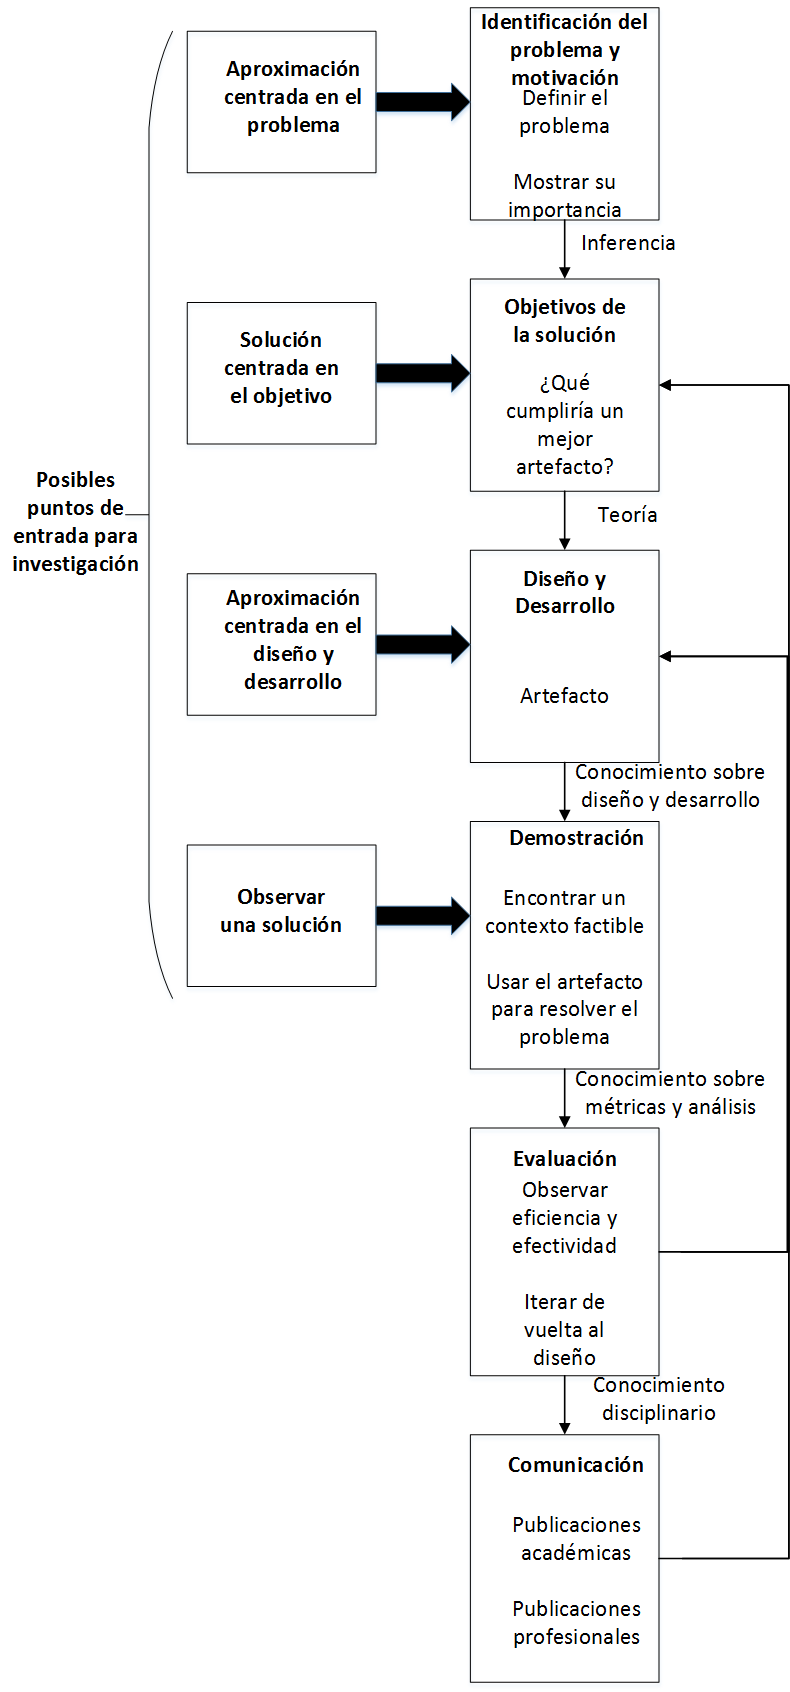
\includegraphics[width=0.5\textwidth]{img/DSRPmodel.png}
\end{center}
\caption{Modelo del proceso de investigación en ciencias del diseño. Tomado de \citep{Peffers2006}}
\label{fig: dsrp}
\end{figure}

Los resultados de la primera y segunda actividad fueron expresados en la introducción de este documento. El diseño y desarrollo incluye determinar las funcionalidades deseadas del artefacto y su arquitectura para luego crear el artefacto en cuestión. Los elementos esenciales que debe poseer una aplicación informática para el OBDA/OBDI fueron sintetizados en el subepígrafe \ref{Acceso e Integración de Datos Basado en Ontologías}. Los artefactos creados serán descritos en los epígrafes siguientes, mientras que la demostración de su eficacia en la solución del problema, así como la observación y medición de su desempeño relativos a las actividades cuatro y cinco del proceso serán expuestas en el Capítulo \ref{Capítulo 3}. Como evidencia de la comunicación a otros investigadores del problema abordado en la investigación y su relevancia, el artefacto creado, su utilidad y su efectividad, se encuentran artículos publicados en revistas y trabajos presentados en eventos por el autor de esta investigación \citep{Tabares-Martin2015,Tabares-Martin2016,Tabares-Martin20161}.

El método propuesto para la Integración de Datos Basada en Ontologías se denomina OntoIntegra. Este método describe el proceso para la integración de los datos almacenados en fuentes de datos estructuralmente heterogéneas en una respuesta conceptualmente homogénea, a partir de la instanciación de una ontología creada para la OBDI. El método se basa en los constructos: consulta sintáctica e instancia de una ontología.

\textbf{Definición 2.1.1} \textit{Una consulta sintáctica es la secuencia textual de instrucciones que permite recuperar información almacenada en al menos una fuente de datos.}

\textbf{Definición 2.1.2} \textit{Sea una ontología compuesta por una parte conceptual (T-Box) y una parte asercional (A-Box). Se denomina instancia de la ontología a su parte asercional.}

\section{OntoIntegra}

\begin{minipage}{\textwidth}

El aporte teórico fundamental de esta investigación es un método para la integración semántica de datos almacenados en fuentes estructuralmente heterogéneas. La figura \ref{fig: metodoOntoIntegra} ilustra el método propuesto, denominado OntoIntegra. Este método describe la obtención de información conceptualmente integrada a través de cinco pasos fundamentales:

\begin{enumerate}
\item Análisis estructural de cada fuente de datos.
\item Análisis semántico de la información almacenada en cada fuente de datos.
\item Instanciación de la ontología para OBDI.
\item Publicación de la instancia de la ontología creada.
\item Consumo por una aplicación informática de la instancia de la ontología creada.
\end{enumerate}

\end{minipage}

\begin{figure}
\begin{center}
	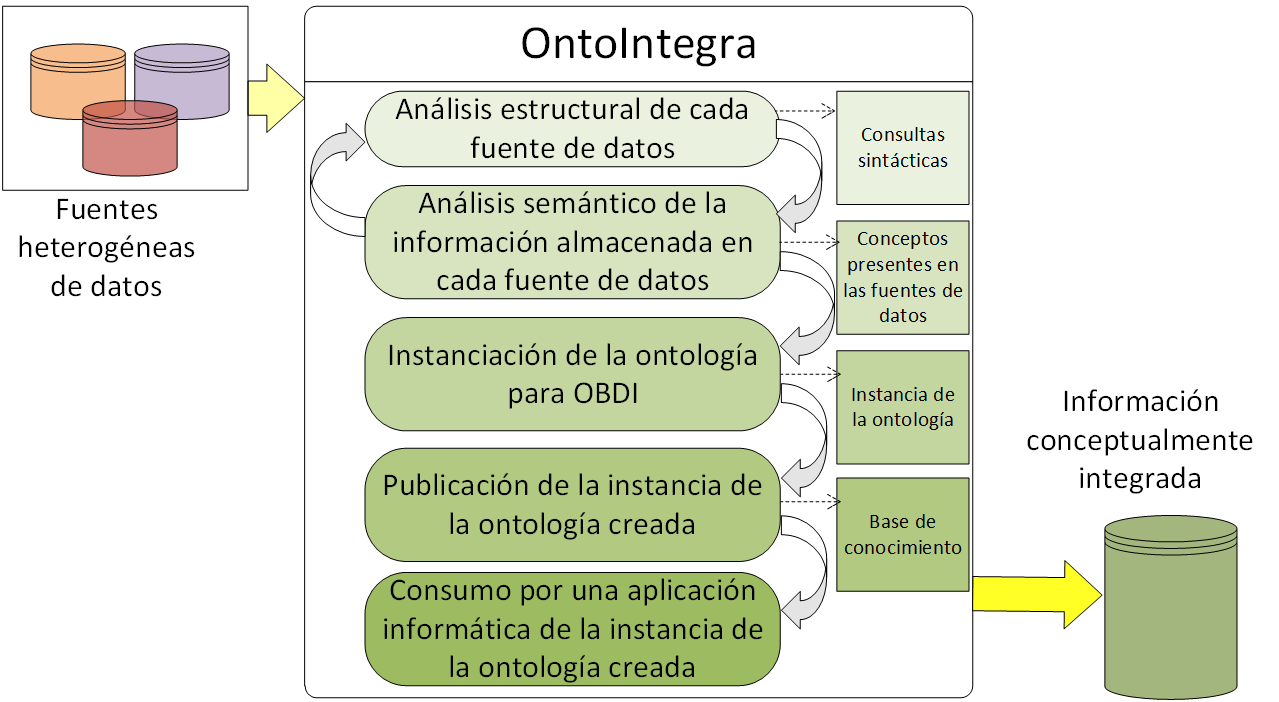
\includegraphics[width=0.8\textwidth]{img/Metodo_OntoIntegra.png}
\end{center}
\caption{Esquema representativo del método OntoIntegra}
\label{fig: metodoOntoIntegra}
\end{figure}


\subsection{Análisis estructural de cada fuente de datos}

El análisis estructural de cada fuente de datos tiene como objetivo identificar la forma en que se encuentran estructurados los datos a recuperar, formulando la consulta sintáctica adecuada a este proceso. En este paso interviene un Experto del dominio, el cual es una persona que conoce en detalle la estructura de los datos gestionados por la fuente de datos en cuestión. En el caso de las bases de datos relacionales, el ``Lenguaje de Consultas Estructurado'' (``Structured Query Language'' - SQL, por sus siglas de acuerdo al término en idioma inglés) constituye el estándar para la recuperación de datos \citep{Eisenberg:1999:SFK:309844.310075}. Este tipo de bases de datos se ha utilizado durante más de dos décadas \citep{BUCKLES1993660,Hristidis2002670,10.1007/978-981-10-8276-4_22}, por lo que gran parte de los datos almacenados a nivel mundial se encuentran sobre el modelo relacional.

Las bases de datos no relacionales, incluyendo las jerárquicas, orientadas a grafos y orientadas a objetos existen desde finales de la década de 1960 \citep{Leavitt2010}. Con el surgimiento y desarrollo de la Web 3.0, las bases de datos orientadas a grafos que soportan el modelo de datos RDF han ganado popularidad \citep{Zaki2017,BRISABOA2017106}. El lenguaje ``Protocolo SPARQL y Lenguaje de Consulta RDF'' (``SPARQL Protocol and RDF Query Language'' - SPARQL, por sus siglas de acuerdo al término en idioma inglés) es la recomendación del ``Consorcio de la World Wide Web'' (``World Wide Web Consortium'' - W3C, por sus siglas de acuerdo al término en idioma inglés) para la consulta sobre grafos RDF \citep{W3CSPARQLWorkingGroup2013}.

Cada vez son más los servicios que se publican en la Web usando la ``Transferencia de estado representacional'' (``Representational state transfer'' - REST, por sus siglas de acuerdo al término en idioma inglés) \citep{Pautasso2014}. El estilo de arquitectura REST enfatiza la escalabilidad de las interacciones entre los componentes de las aplicaciones informáticas y promueve la reutilización de los componentes reduciendo su acoplamiento \citep{Pautasso2014}. Resulta posible considerar aplicaciones externas que exponen sus datos a través de REST como fuentes de datos. En este caso, el análisis estructural de la fuente de datos se centraría en la estructura sintáctica que debe poseer la petición a formular para extraer los datos a integrar.

El Experto de dominio en este paso analiza cómo están físicamente distribuidos los datos que se pretenden integrar en las fuentes de datos que los almacenan. Posteriormente formula las consultas sintácticas que permitirán recuperar dichos datos utilizando los constructos definidos para este fin en las fuentes de datos a encuestar.

\subsection{Análisis semántico de la información almacenada en cada fuente de datos}

En el análisis semántico de la información almacenada en cada fuente de datos se determinan los conceptos contenidos en las mismas cuyos datos asociados se desean recuperar. En este paso interviene un Experto del dominio y un Ingeniero de conocimiento. El Ingeniero de conocimiento tiene la función de traducir los elementos presentes en una fuente de datos a conceptos comprensibles por un usuario externo.

En este paso un Usuario de conceptualización requiere ciertos conceptos sobre un dominio específico, esta petición se la realiza a un Experto del dominio. El Experto del dominio determina exactamente qué elementos del dominio son los que necesita el Usuario de conceptualización y se lo informa al Ingeniero de conocimiento. El Ingeniero de conocimiento modela conceptualmente los elementos recibidos en términos conocidos por el Usuario de conceptualización y retorna la conceptualización elaborada. Este proceso se ilustra en la figura \ref{fig: conceptsExtraction}.

\textbf{Proceso de desarrollo de la ontología según la metodología METHONTOLOGY}

El proceso de desarrollo de una ontología se refiere a cuáles actividades deben realizarse al construir una ontología \citep{Gomez-Perez:2007:OEE:1199560}. La metodología METHONTOLOGY propone la realización de tres categorías de actividades que se ilustran en la figura \ref{fig: methontology}.

\begin{figure}
\begin{center}
	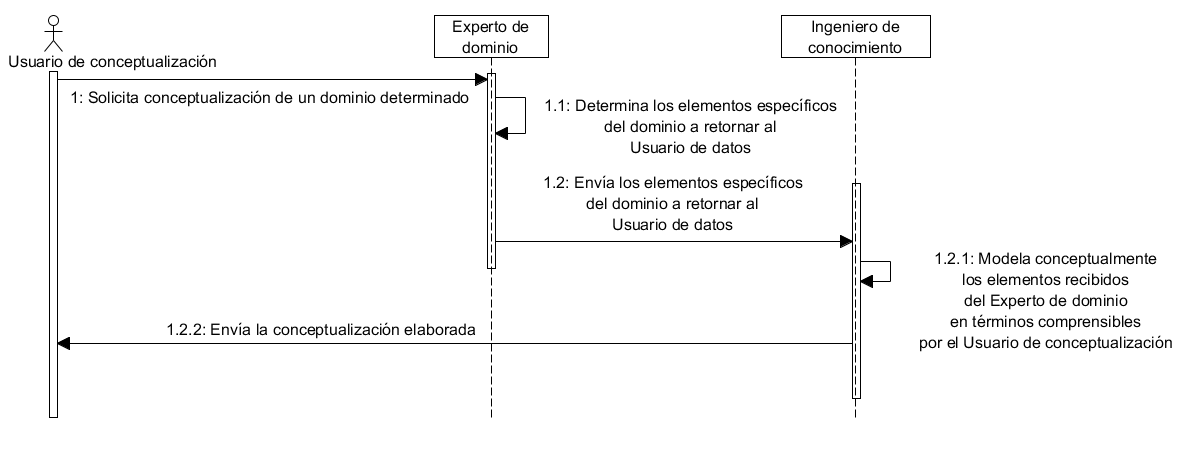
\includegraphics[width=1\textwidth]{img/conceptsExtraction.png}
\end{center}
\caption{Secuencia realizada en el paso Análisis semántico de la información almacenada en cada fuente de datos}
\label{fig: conceptsExtraction}
\end{figure}

\begin{figure}
\begin{center}
	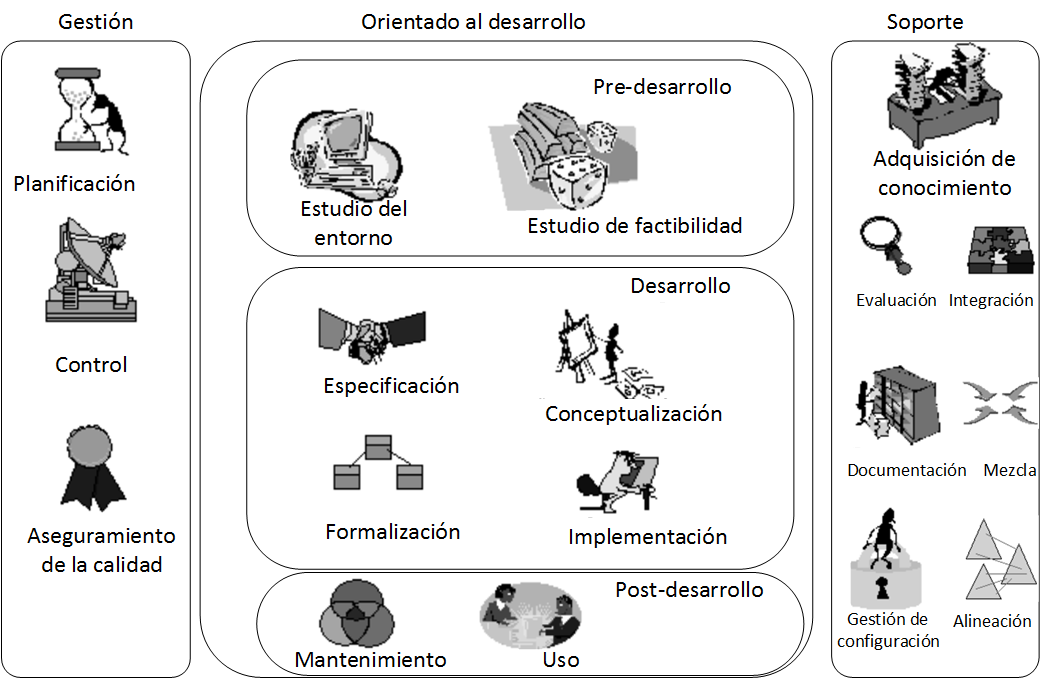
\includegraphics[width=0.8\textwidth]{img/Diagrama_METHONTOLOGY.png}
\end{center}
\caption{Proceso de desarrollo de una ontología. Tomado de \citep{Gomez-Perez:2007:OEE:1199560}}
\label{fig: methontology}
\end{figure}

Las actividades de gestión incluyen la planificación, el control y el aseguramiento de la calidad. La actividad de \textit{planificación} identifica las tareas a desarrollar, su prioridad, el tiempo y los recursos para llevarlas a cabo. El resultado de esta actividad se ilustra en la figura \ref{fig: planificacion}. La actividad de \textit{control} garantiza que las tareas planificadas se completen conforme a la manera en que se diseñaron. Finalmente, la actividad de \textit{aseguramiento de la calidad} verifica que la calidad de cada artefacto generado (la ontología, la aplicación informática y la documentación) sea satisfactoria \citep{Gomez-Perez:2007:OEE:1199560}. El cumplimiento de la actividad de \textit{aseguramiento de la calidad} fue certificado por el tribunal que evaluó el ejercicio de culminación de estudios titulado ``AUCTORITAS 2.0: Sistema de apoyo para el control de autoridades''.

\begin{figure}
\begin{center}
	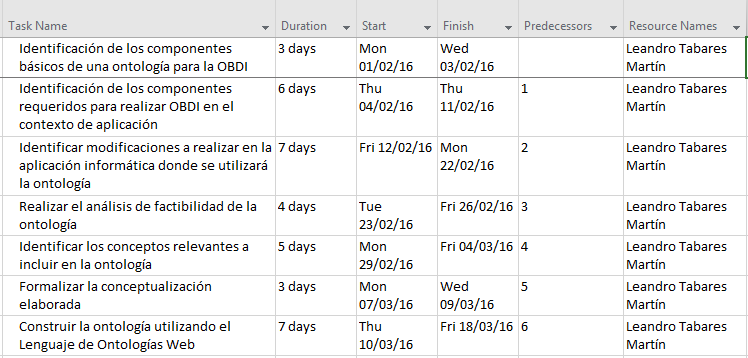
\includegraphics[width=0.8\textwidth]{img/planificacionTareas.PNG}
\end{center}
\caption{Planificación de las tareas para el desarrollo de la ontología}
\label{fig: planificacion}
\end{figure}

Las actividades orientadas al desarrollo de la ontología se agrupan en actividades pre-desarrollo, actividades de desarrollo y actividades post-desarrollo. Durante las actividades pre-desarrollo se realiza un \textit{estudio del entorno} con el fin de conocer las plataformas en las que se utilizará la ontología, las aplicaciones en las que la ontología será integrada, entre otros detalles. Como resultado de esta actividad se determinó que la ontología se utilizaría en una plataforma Java, al ser integrada en la aplicación informática AUCTORITAS versión 2.0. También, durante las actividades pre-desarrollo se lleva a cabo un \textit{análisis de factibilidad} que debe responder a preguntas como: ¿Es posible construir la ontología? ¿Es factible construir la ontología? \citep{Gomez-Perez:2007:OEE:1199560}.

Una vez en el desarrollo, la actividad \textit{especificación} determina el por qué la ontología se está construyendo, para qué se usará y quiénes son los usuarios finales. La \textit{conceptualización} estructura el dominio de conocimiento en forma de modelos significativos al nivel de conocimiento, el resultado de esta actividad se ilustra en la figura \ref{fig: mapaConceptual}. 

\begin{figure}[H]
\begin{center}
	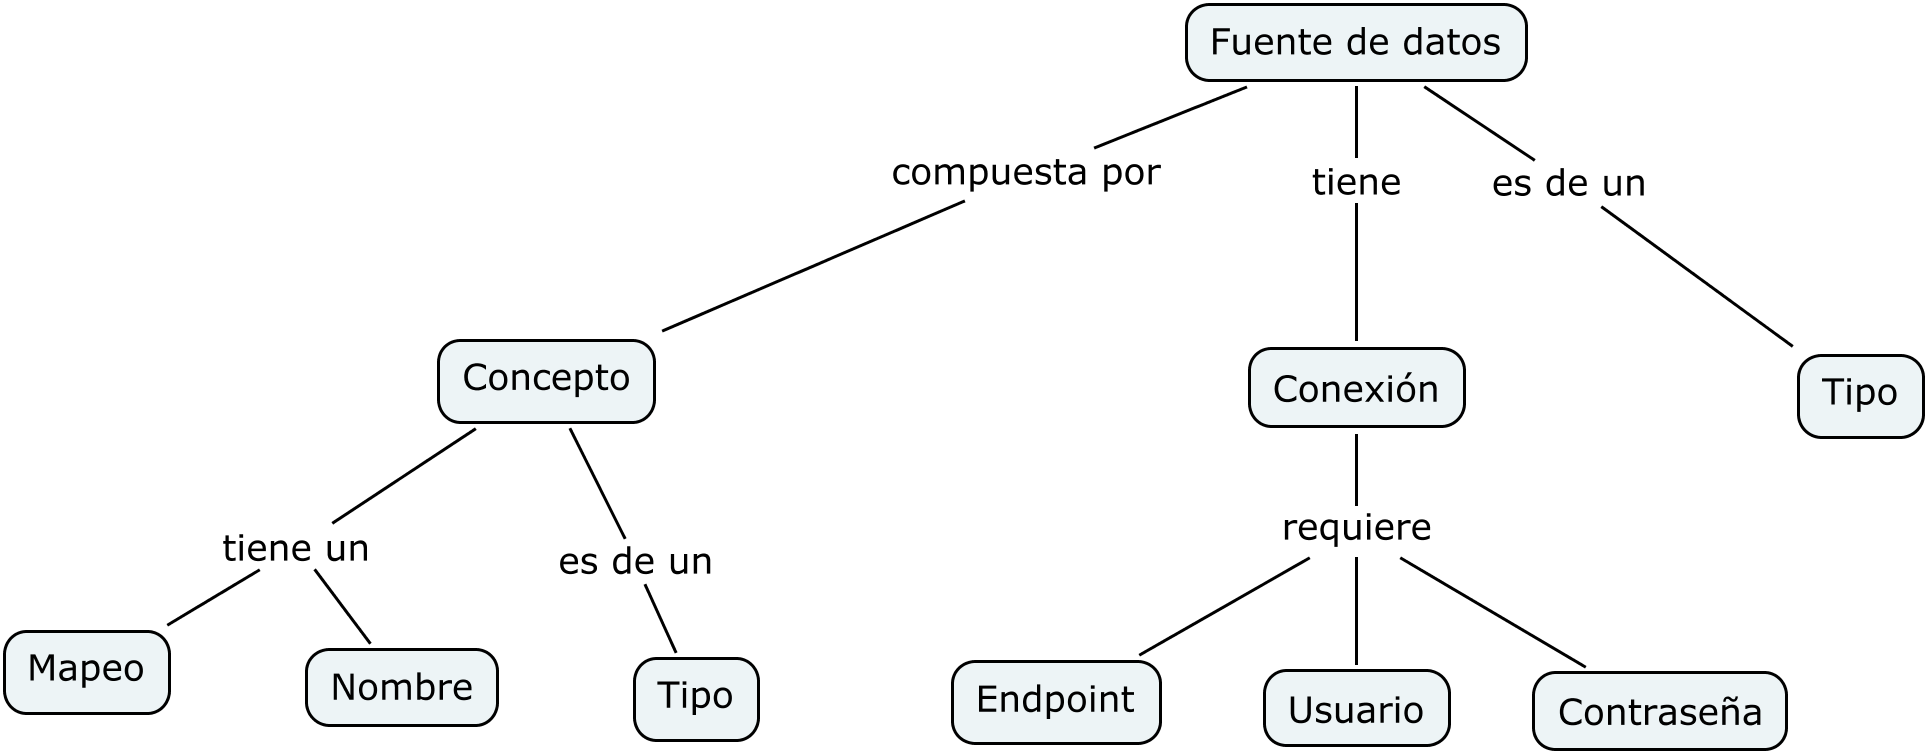
\includegraphics[width=0.8\textwidth]{img/mapaConceptual.png}
\end{center}
\caption{Conceptualización de los elementos del dominio de conocimiento}
\label{fig: mapaConceptual}
\end{figure}

La actividad \textit{formalización} transforma el modelo conceptual en un modelo formal o semi-computable, por medio de la utilización de los constructos definidos en la Lógica Descriptiva \citep{Baader2003}. Para formalizar la conceptualización elaborada se decidió desarrollar la ontología que se ilustra en la figura \ref{onto:hdrm}. Esta ontología cumple con el requisito definido por \cite{Calvanese2017}, el cual especifica que los elementos básicos que debe poseer una ontología diseñada con el propósito de permitir la OBDI son los definidos en la ontología \ref{onto:elementosBasicosOntologiaOBDI}.\\

\begin{minipage}{\textwidth}
$Concept \ \equiv \ Thing \ \sqcap \ \exists  mappedTo.Literal \ \sqcap \ =1 mappedTo \ \sqcap \exists  type.Literal \ \sqcap \ =1 type \ \sqcap \ \exists name.String \sqcap \ =1 name$ \\
$Connection \ \equiv \ Thing \ \sqcap \ \exists endpoint.Literal \ \sqcap \ =1 endpoint \ \sqcap \ \forall user.String \ \sqcap \ \forall password.String $ \\
$Datasource \ \equiv \ Thing \ \sqcap \ \exists composedBy.Concept \ \sqcap \ \exists has.Connection \ \sqcap \ =1 has \ \sqcap \ type.Literal \ \sqcap \ =1 type$ \\
\captionof{figure}{T-Box de la ontología desarrollada}
\label{onto:hdrm}
\end{minipage}\\

\begin{equation}
Concepto \equiv Thing \sqcap \exists mapeo.Literal
\label{onto:elementosBasicosOntologiaOBDI}
\end{equation}

La actividad de \textit{implementación} construye modelos computables en un lenguaje de ontologías \citep{Gomez-Perez:2007:OEE:1199560}. Este modelo se construyó utilizando el Lenguaje de Ontologías Web por medio de la herramienta Protégé y se ilustra en la figura \ref{fig: ontologiaProtege}.

\begin{figure}
\begin{center}
	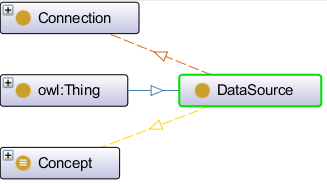
\includegraphics[width=0.5\textwidth]{img/ontologiaProtege.png}
\end{center}
\caption{Clases de la ontología construida con la herramienta Protégé}
\label{fig: ontologiaProtege}
\end{figure}

Durante el post-desarrollo, la actividad de \textit{mantenimiento} actualiza y corrige la ontología de ser necesario. También en esta fase la ontología es reutilizada por otras ontologías o aplicaciones \citep{Gomez-Perez:2007:OEE:1199560}.

Finalmente, las actividades de soporte incluyen una serie de actividades que se realizan al mismo tiempo que las orientadas al desarrollo. Ellas incluyen la adquisición de conocimiento, evaluación, integración, mezcla, alineación, documentación y gestión de configuración. El objetivo de la actividad de \textit{adquisición de conocimiento} es obtener el conocimiento de expertos del dominio a través de algún tipo de procedimiento (semi)automático, lo que se conoce como aprendizaje ontológico. La actividad de \textit{evaluación} realiza un juicio técnico de las ontologías, sus entornos de aplicaciones informáticas asociados, así como de la documentación. Este juicio se realiza con respecto a un marco de referencia durante cada etapa y entre etapas durante el ciclo de vida de la ontología. La actividad de \textit{integración} se requiere cuando se construye la ontología a partir de la reutilización de otras ontologías \citep{Gomez-Perez:2007:OEE:1199560}.

Otra actividad de soporte es la \textit{mezcla}, que consiste en la obtención de una ontología a partir de diferentes ontologías del mismo dominio. La actividad de \textit{alineación} establece diferentes tipos de mapeos entre las ontologías  involucradas. Por otra parte, la actividad de \textit{documentación} detalla, clara y exhaustivamente cada una de las etapas completadas y los productos generados. La \textit{gestión de configuración} almacena todas las versiones de la documentación y del código de la ontología para controlar los cambios.

\subsection{Instanciación de la ontología para la integración de datos}

\cite{JANNACH2009136} han demostrado que las ontologías de dominio pueden apoyar la extracción de conocimiento, lo que significa que el problema de extracción de información puede ser generalizado al problema de encontrar e insertar información que concuerde con una ontología en la base de conocimiento de un sistema, este proceso se conoce como ``instanciación de la ontología'' o ``poblado de la ontología''. Entonces la ontología instanciada puede servir como base para el desarrollo de servicios de conocimiento en la Web Semántica \citep{1179189}.

La instanciación de una ontología es un proceso costoso y que consume tiempo \citep{10.1007/978-0-387-87685-6_30}, por esta razón existen enfoques automáticos \citep{1179189,JANNACH2009136} y semi-automáticos \citep{10.1007/978-0-387-87685-6_30}. La instanciación de la ontología para OBDI consiste en la representación de los conceptos identificados en el paso anterior acorde a la terminología definida por la ontología seleccionada. Debido al alto nivel de detalle que implica instanciar una ontología para OBDI se escogió realizar este proceso manualmente. 

Para la instanciación manual de una ontología es posible apoyarse en un editor de ontologías. La tabla \ref{tab: editores} sintetiza características de varios editores de ontologías.

\begin{table}
\begin{tabular}{|c|c|c|c|c|c|}
\hline 
Herramienta & Versión & Propietario / & Características / & Lenguaje & Libre \\ 
 &  & Desarrollador & Limitaciones & primario & Libre \\
\hline 
Adaptiva & - & Universidad Sheffield & Adquisición de & Java & Sí \\ 
 &  &  & conocimiento &  &  \\
\hline 
Semantic-works 2012 & 2012 & Altova & Editor OWL + RDFS & Java & No \\ 
\hline 
Conzilla & 2.2 & Grupo de investigaciones & Navegador de  & Java & Sí \\ 
 & & de gestión del conocimiento & conceptos &  &  \\
\hline 
HOZO & 5.6 & Universidad de & Amigable al & Java & Sí \\ 
 & & Osaka & usuario & & \\
\hline 
Protégé & 5.5.0 & Universidad de Stanford & Herencia múltiple & Java & Sí \\ 
\hline 
\end{tabular} 
\caption{Editores de ontologías}
\label{tab: editores}
\end{table}

Un ejemplo de instanciación se ilustra en la figura \ref{onto:auctoritasDescription}, en la que se utilizó la variable syntacticQuery con el objetivo de facilitar su comprensión. Esta variable se refiere a una consulta sintáctica formulada en un lenguaje de consulta (por ejemplo: SQL, SPARQL, una petición REST, entre otros).

\begin{minipage}{\textwidth}
$Datasource(PostgreSQL), \ has(PostgreSQL, postgresConnection), \ type(PostgreSQL,local)$ \\
$composedBy(PostgreSQL, autorPersonalPostgres).$ \\
$Concept(autorPersonalPostgres), \ mappedTo(autorPersonalPostgres, syntacticQuery),$ \\
$type(autorPersonalPostgres,AUTORPERSONAL), \ name(autorPersonalPostgres, Autor \ Personal).$\\
$Connection(postgresConnection), \ user(postgresConnection,postgres),$ \\
$password(postgresConnection,admin),$ \\
$endpoint(postgresConnection, jdbc{:}postgresql{:}//localhost{:}5432/Autoridades).$ \\
$Datasource(VIVO), \ has(VIVO, vivoConnection), \ composedBy(VIVO,institution),$ \\
$composedBy(VIVO,autorPersonalVivo), \ type(PostgreSQL,http).$ \\
$Concept(institution), \ mappedTo(institution,syntacticQuery), \ name(institution, Institution)$ \\
$type(institution,AUTORCORPORATIVO).$\\
$Concept(autorPersonalVivo), \ mappedTo(autorPersonalVivo, syntacticQuery),$ \\
$type(autorPersonalVivo, AUTORPERSONAL), name(autorPersonalVivo, Autor \ Personal).$ \\
$Connection(vivoConnection),$\\
$endpoint(vivoConnection, $\\
$http{:}//localhost{:}8080/vivo/api/sparqlQuery?email{=}vivoroot@mydomain.edu\&password{=}zas123..).$\\
$Datasource(ORCID), \ composedBy(ORCID,autorPersonalOrcid), \ has(ORCID,orcidConnection),$ \\
$type(ORCID, orcid).$ \\
$Concept(autorPersonalOrcid), \ mappedTo(autorPersonalOrcid, syntacticQuery),$\\
$type(autorPersonalOrcid,AUTORPERSONAL), \ name(autorPersonalOrcid, Autor \ Personal.)$ \\
$Connection(orcidConnection),$\\
$endpoint(orcidConnection, https{:}//pub{.}orcid{.}org/v1{.}2/search/orcid{-}bio/?q{=}).$\\
$Datasource(AGROVOC), \ composedBy(AGROVOC, agrovocConcept),$\\
$has(AGROVOC, virtuosoConnection), \ type(AGROVOC,http).$ \\
$Concept(agrovocConcept), \ mappedTo(agrovocConcept, syntacticQuery), $\\
$type(agrovocConcept, CONTROLEDTERMS), \ name(agrovocConcept, Termino \ Controlado)$\\
$Connection(virtuosoConnection),$
$endpoint(virtuosoConnection, http{:}//localhost{:}8890/sparql).$\\
$Datasource(ACM), \ composedBy(ACM, acmConcept), \ has(ACM, virtuosoConnection),$\\
$type(ACM,http).$ \\
$Concept(acmConcept), \ mappedTo(acmConcept,syntacticQuery),$\\
$type(acmConcept,CONTROLEDTERMS),  \ name(acmConcept, Termino \ Controlado)$\\
\captionof{figure}{A-Box de la ontología desarrollada}
\label{onto:auctoritasDescription}
\end{minipage}

\subsection{Publicación de la instancia de la ontología creada}

Uno de los principales retos que se enfrentan en la Web Semántica es que las ontologías típicamente se publican como ficheros sin soporte para utilizarlos en aplicaciones \citep{viljanen2008publishing}. Los almacenes de tripletas RDF constituyen un tipo de bases de datos basadas en grafos, lo que les permite almacenar datos en forma de redes de objetos vinculados entre sí. Las bases de datos de este tipo son  capaces de gestionar consultas semánticas y utilizar inferencias para descubrir nueva información implícita en los datos almacenados y sus relaciones.

La publicación de la instancia de la ontología creada se refiere a su carga en un almacén de tripletas RDF. Este paso permite compartir en línea la instancia, haciéndola reutilizable por otras aplicaciones que requieran acceder a las fuentes de datos descritas. Los elementos descritos en una ontología publicada en un almacén de tripletas RDF son accesibles mediante consultas SPARQL, beneficiándose de las características de este tipo de bases de datos y de las potencialidades del lenguaje de consultas.

\subsection{Consumo por una aplicación informática de la instancia de la ontología creada}

El consumo por una aplicación informática de la instancia de la ontología creada permite, a partir de la descripción de los términos de la ontología, obtener su instanciación y utilizarla para recuperar los datos requeridos. En este paso se utiliza la T-Box de la ontología como base para la interpretación semántica de la estructura de la fuente de datos a encuestar.

La A-Box de la ontología brinda a la aplicación informática los datos necesarios para gestionar la conexión a la fuente de datos. A su vez, contiene los conceptos relevantes a recuperar y las consultas sintácticas que posibilitan este proceso.

\section{Conclusiones del capítulo}

El paradigma de las ciencias del diseño permitió definir el artefacto a generar como aporte teórico principal de la investigación. El proceso utilizado para la investigación en ciencias del diseño condujo las actividades a realizar como parte del presente trabajo.

El método creado permite la integración de datos almacenados en fuentes estructuralmente heterogéneas, brindando una guía a los especialistas encargados de este proceso. La utilización de la metodología para el desarrollo de ontologías seleccionada, orientó satisfactoriamente el proceso de desarrollo de la ontología que se propone como parte del método.





